\section{18. Übungsblatt}

\subsection{Aufgabe 18.1}

\subsubsection{(a)}
\begin{align*}
&\lim_{x\rightarrow 1}\frac{\ln(x)}{x-\sqrt{x}}\\
&=\lim_{x\rightarrow1}\frac{\frac{1}{x}}{1-\frac{1}{2\sqrt{x}}}=\frac{1}{\frac{1}{2}}=2
\end{align*}

\subsubsection{(b)}
\begin{align*}
&\lim_{x\rightarrow0}\frac{\ln(\cos(x))}{x^2}\\
&=\lim\frac{\frac{1}{\cos(x)}\cdot(-\sin(x))}{2x}\\
&=\lim\frac{-\tan(x)}{2x}\\
&=\lim\frac{-\frac{1}{\cos^2(x)}}{2}=\frac{-1}{2}
\end{align*}

\subsubsection{(c)}
\begin{align*}
&\lim_{x\rightarrow0}x^{\frac{1}{1-x}}\\
&=(e^{\lim \ln(x)})^{\frac{1}{1-x}}\\
&=e^{\lim\ln(x)\cdot\frac{1}{1-x}}\\
&\lim\frac{\ln(x)}{1-x}=\lim_{x\rightarrow1}\frac{\frac{1}{x}}{-1}=-1
\end{align*}

\subsubsection{(d)}
\begin{align*}
&\lim_{x\rightarrow0}\frac{(1-x)^\alpha-(1-\alpha x)}{x^2}="\frac{0}{0}"\\
&=\lim\frac{-\alpha(1-x)^{\alpha-1}+\alpha}{2x}="\frac{0}{0}"\\
&=\lim\frac{\alpha(\alpha-1)(1-x)^{\alpha-2}}{2}\\
&=\frac{\alpha(\alpha-1)}{2}
\end{align*}

\newpage

\subsubsection{(e)}
\begin{align*}
&\lim_{x\rightarrow\infty}x\ln(1+\frac{1}{x})="\infty\cdot0"\\
&=\lim\frac{\ln(1-\frac{1}{x})}{\frac{1}{x}}="\frac{0}{0}"\\
&=\lim\frac{-\frac{1}{1+\frac{1}{x}}x^{-2}}{-x^{-2}}=\lim\frac{1}{1+\frac{1}{x}}=1
\end{align*}

\subsubsection{(f)}
\begin{align*}
&\lim_{x\downarrow0}(\cot(x))^{\sin(x)}\\
&=\lim\exp(\frac{\ln(\cot(x))}{\frac{1}{\sin(x)}})="\frac{\infty}{\infty}"\\
&=\exp\bigg(\lim\frac{-\frac{1}{\cot(x)}\cdot\frac{1}{\sin^2(x)}}{-\sin^{-2}(x)\cdot\cos(x)}\bigg)\\
&=\exp(\lim\frac{\frac{\sin(x)}{\cot(x)}}{\cot(x)})\\
&=\exp(\lim\frac{\sin(x)}{\cot^2(x)})=1
\end{align*}

\newpage

\subsection{Aufgabe 18.2}

\subsection{Aufgabe 18.3}

\subsection{Aufgabe 18.4}

\subsection{Aufgabe 18.5(H)}

\subsection{Aufgabe 18.6(H)}

\newpage

\subsection{Tutorium}

$\lim_{x\rightarrow x_0}\frac{f}{g}\overset{Formel}{=}\frac{\lim f}{\lim g}=\frac{\infty}{\infty}oder\frac{0}{0}$,dann

Falls $\lim_{x\rightarrow x_0}\frac{f'}{g'}$ ex., dann ex. auch $\lim_{x\rightarrow x_0}\frac{f}{g}$, und die sind gleich.

\begin{exmp}
$\lim_{x\rightarrow\infty}\frac{e^x+e^{-x}}{e^x-e^{-x}}=\frac{\infty}{\infty}$, aber $\lim_{x\rightarrow\infty}\frac{e^x-e^{-x}}{e^x+e^{-x}}=\frac{\infty}{\infty}$ auch.

Es gilt $\lim_{x\rightarrow\infty}\frac{e^x}{e^x}\frac{1+e^{-2x}}{1-e^{-2x}}=\frac{\lim 1+e^{-2x}}{\lim 1-e^{-2x}}=1$
\end{exmp}

\begin{definition}[HP]
\begin{equation*}
I\subseteq\mathbb{R},\ a\in I\ \mbox{sei HP von}\ I=\left\{
\begin{array}{lcl}
\forall\varepsilon>0:\ B(a,\varepsilon)\setminus\{a\}\cap I\neq\emptyset\\
\mbox{Ex ex. Folge}\ (x_n)\ \mbox{in}\ I\setminus\{a\}\ \mbox{mit}\ \lim_{n\rightarrow\infty}x_n=a
\end{array}
\right.
\end{equation*}
\end{definition}

$h(x)=f(x)g(x)$:

Sei $(p_n)$ ein Folge in $\mathbb{R}\setminus\{0\}$  mit $p_n\rightarrow0$, und $x_n=a+p_n\in I$ für alle $n\in\mathbb{N}$
\begin{align*}
\Rightarrow\frac{h(a+p_n)-h(a)}{p_n}&=\frac{f(a+p_n)g(a+p_n)-f(a)g(a)}{p_n}\\
&=\frac{f(a+p_n)g(a+p_n)-f(a)g(a+p_n)}{p_n}\\
&=g(a+p_n)\frac{f(a+p_n)-f(a)}{p_n}\\
(n\rightarrow\infty)&=g(a)f'(a)
\end{align*}

Da dies für jede Folge $(p_n)$, dieser Art gilt.\\

\begin{definition}[Norm]
$x=(x_1,\cdots,x_n)\in\mathbb{R}^n\ od.\ \mathbb{C}^n$,
\begin{equation*}
||x||_p:=\bigg(\sum_{k=1}^n|x_k|^p\bigg)^{\frac{1}{p}},\ p\in[1,\infty)
\end{equation*}
\begin{equation*}
||x||_\infty:=\max\{|x_1|,\cdots,|x_n|\}
\end{equation*}
\end{definition}

\center


\tikzset{every picture/.style={line width=0.75pt}} %set default line width to 0.75pt        

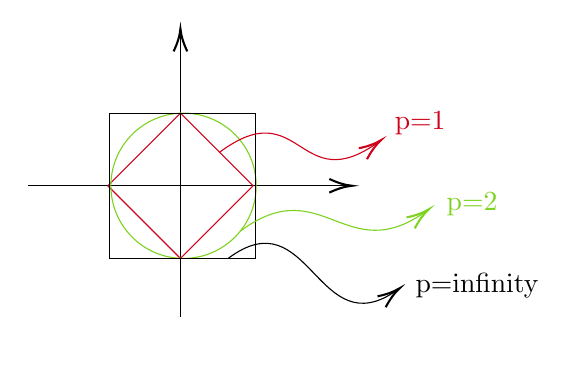
\begin{tikzpicture}[x=0.75pt,y=0.75pt,yscale=-1,xscale=1]
%uncomment if require: \path (0,300); %set diagram left start at 0, and has height of 300

%Straight Lines [id:da08558939251119768] 
\draw    (235.67,147) -- (389.67,147) ;
\draw [shift={(391.67,147)}, rotate = 180] [color={rgb, 255:red, 0; green, 0; blue, 0 }  ][line width=0.75]    (10.93,-3.29) .. controls (6.95,-1.4) and (3.31,-0.3) .. (0,0) .. controls (3.31,0.3) and (6.95,1.4) .. (10.93,3.29)   ;
%Straight Lines [id:da7594655962770807] 
\draw    (309,210.33) -- (309,73.33) ;
\draw [shift={(309,71.33)}, rotate = 90] [color={rgb, 255:red, 0; green, 0; blue, 0 }  ][line width=0.75]    (10.93,-3.29) .. controls (6.95,-1.4) and (3.31,-0.3) .. (0,0) .. controls (3.31,0.3) and (6.95,1.4) .. (10.93,3.29)   ;
%Shape: Diamond [id:dp39135482364715646] 
\draw  [color={rgb, 255:red, 208; green, 2; blue, 27 }  ,draw opacity=1 ] (309,112) -- (344,147) -- (309,182) -- (274,147) -- cycle ;
%Shape: Circle [id:dp1752761740956985] 
\draw  [color={rgb, 255:red, 126; green, 211; blue, 33 }  ,draw opacity=1 ] (275.5,147) .. controls (275.5,127.67) and (291.17,112) .. (310.5,112) .. controls (329.83,112) and (345.5,127.67) .. (345.5,147) .. controls (345.5,166.33) and (329.83,182) .. (310.5,182) .. controls (291.17,182) and (275.5,166.33) .. (275.5,147) -- cycle ;
%Shape: Square [id:dp6636179969902987] 
\draw   (275,112) -- (345,112) -- (345,182) -- (275,182) -- cycle ;
%Curve Lines [id:da932883061649141] 
\draw [color={rgb, 255:red, 208; green, 2; blue, 27 }  ,draw opacity=1 ]   (327.67,131) .. controls (367.27,101.3) and (365.7,153.93) .. (404.48,125.87) ;
\draw [shift={(405.67,125)}, rotate = 143.13] [color={rgb, 255:red, 208; green, 2; blue, 27 }  ,draw opacity=1 ][line width=0.75]    (10.93,-3.29) .. controls (6.95,-1.4) and (3.31,-0.3) .. (0,0) .. controls (3.31,0.3) and (6.95,1.4) .. (10.93,3.29)   ;
%Curve Lines [id:da161535006788452] 
\draw [color={rgb, 255:red, 126; green, 211; blue, 33 }  ,draw opacity=1 ]   (337.67,169) .. controls (377.27,139.3) and (388.44,187.35) .. (427.48,159.21) ;
\draw [shift={(428.67,158.33)}, rotate = 143.13] [color={rgb, 255:red, 126; green, 211; blue, 33 }  ,draw opacity=1 ][line width=0.75]    (10.93,-3.29) .. controls (6.95,-1.4) and (3.31,-0.3) .. (0,0) .. controls (3.31,0.3) and (6.95,1.4) .. (10.93,3.29)   ;
%Curve Lines [id:da69555676469067] 
\draw    (332,182) .. controls (371.6,152.3) and (374.61,224.86) .. (413.48,197.2) ;
\draw [shift={(414.67,196.33)}, rotate = 143.13] [color={rgb, 255:red, 0; green, 0; blue, 0 }  ][line width=0.75]    (10.93,-3.29) .. controls (6.95,-1.4) and (3.31,-0.3) .. (0,0) .. controls (3.31,0.3) and (6.95,1.4) .. (10.93,3.29)   ;

% Text Node
\draw (411,110) node [anchor=north west][inner sep=0.75pt]  [color={rgb, 255:red, 208; green, 2; blue, 27 }  ,opacity=1 ] [align=left] {p=1};
% Text Node
\draw (436,149) node [anchor=north west][inner sep=0.75pt]  [color={rgb, 255:red, 126; green, 211; blue, 33 }  ,opacity=1 ] [align=left] {p=2};
% Text Node
\draw (421,188) node [anchor=north west][inner sep=0.75pt]   [align=left] {p=infinity};


\end{tikzpicture}
